Nick Vosseteig

2014-11-14

building, wiring, programming

\begin{tabular}{|p{5cm}|p{5cm}|}
 \hline
 building&
We built two spinners, one to intake and one to launch balls up a ramp and built a ramp.
 \\
 \hline
wiring&
David and I took the wires off in order to build and installed power poles into our wiring. We then reattached the wiring.
 \\
 \hline
programming&
I changed the code to accomodate the new wiring and the new spinner.
 \\
 \hline
\end{tabular}

\section*{building}
This week we built an intake device and a spinner. However, upon testing we decided that this setup was not optimal due to problems between the two spinners. We decided to try removing them and making a single, larger spinner that we can use both as an intake, and a launcher.
\section*{Wiring}
This week David and I worked on the wiring. We added power poles onto the wiring and then reattached it to the robot. Here is what the wiring looked like when it was not attached to the robot:
\begin{center}
 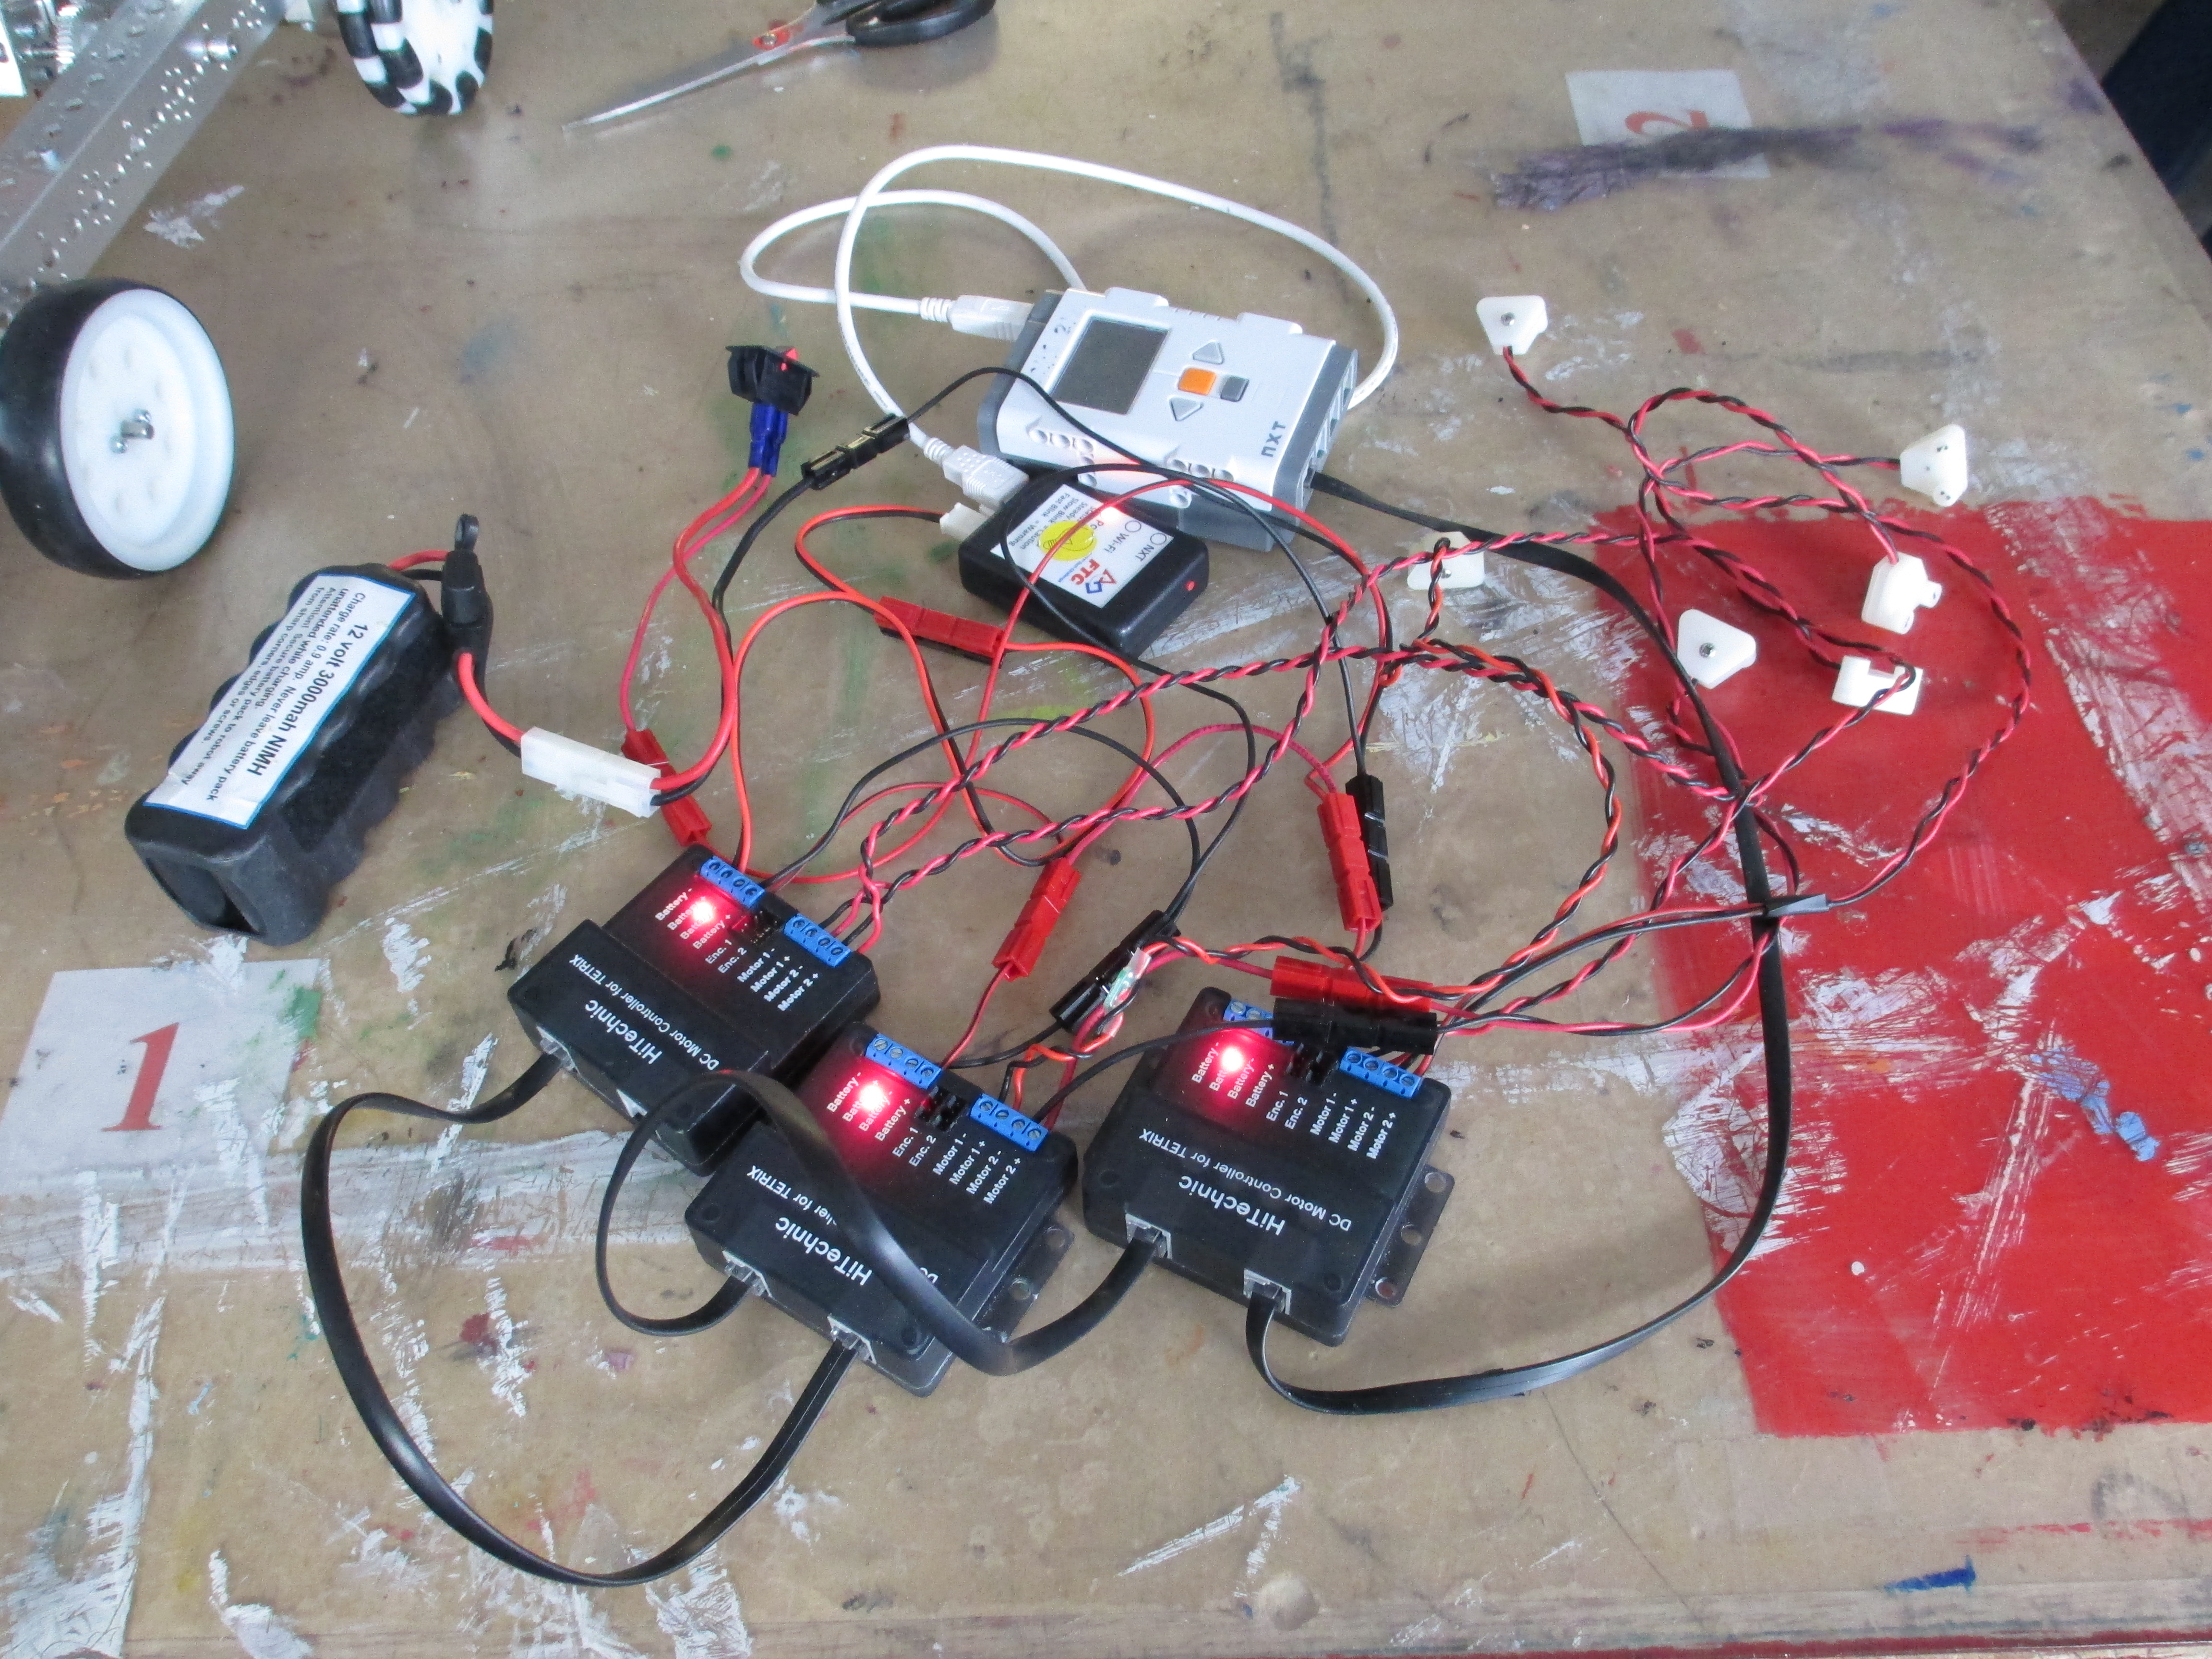
\includegraphics[width=215px]{./Entries/Images/wiring1.jpg}
\end{center}